\documentclass[../../norme-di-progetto.tex]{subfiles}

\begin{document}

\subsubsection{Finalità}%
\label{subs:sviluppo/finalita}

GruppOne istanzia il processo di sviluppo per realizzare il prodotto richiesto dal proponente.

\subsubsection{Descrizione}%
\label{subs:sviluppo/descrizione}

Il processo di sviluppo fissa quali sono gli obiettivi dello sviluppo, dalla creazione alla consegna del prodotto finale.

Raggruppa le seguenti attività:
\begin{itemize}
  \item Implementazione del processo
  \item Analisi dei requisiti del sistema
  \item Progettazione architetturale del sistema
  \item Analisi dei requisiti del software
  \item Progettazione architetturale del software
  \item Progettazione di dettaglio del software
  \item Codifica e test di unità del software
  \item Integrazione del software
  \item Test di integrazione
  \item Integrazione del sistema
  \item Test di sistema
  \item Installazione del software
  \item Supporto all'accettazione del software.
\end{itemize}

\subsubsection{Attività}%
\label{subs:sviluppo/attivita}

% Implementazione del processo
\paragraph{Implementazione del processo}%
\label{par:sviluppo/implementazione_del_processo}

L'implementazione del processo si articola nei seguenti compiti:

\begin{itemize}
  \item Definire o selezionare un modello del ciclo di vita del software appropriato all'ambito, all'entità e alla complessità del progetto.
  \item È necessario:
        \begin{itemize}
          \item Documentare gli output.
          \item Posizionare gli output nel processo di gestione della configurazione ed eseguire le modifiche di controllo in conformità con esso.
          \item Documentare e risolvere problemi e non conformità riscontrati nei prodotti software.
          \item Eseguire i processi di supporto come specificato nel contratto.
        \end{itemize}
  \item Selezionare, personalizzare e utilizzare gli standard, i metodi, gli strumenti e i linguaggi di programmazione (se non previsti nel contratto) che sono documentati e appropriati per lo svolgimento delle attività di processo di sviluppo.
  \item Sviluppare piani che includano standard, metodi, strumenti, azioni e responsabilità specifici associati con lo sviluppo e la qualificazione di tutti i requisiti, compresa la sicurezza, per lo svolgimento delle attività di processo di sviluppo.
  \item Le componenti non consegnabili possono essere impiegate nello sviluppo o nella manutenzione del software. Tuttavia deve essere garantito che le operazioni di sviluppo e manutenzione del software dopo la sua consegna all'acquirente siano indipendenti dalle componenti citate, altrimenti devono essere anch'esse considerate come consegnabili.
\end{itemize}

% Analisi dei requisiti del sistema
\paragraph{Analisi dei requisiti del sistema}%
\label{par:analisi_dei_requisiti_del_sistema}

L'uso specifico previsto del sistema da sviluppare deve essere analizzato per specificare i requisiti di sistema. La specifica dei requisiti di sistema deve descrivere: funzioni e capacità del sistema; requisiti aziendali, organizzativi e dell'utente; requisiti di sicurezza, di interfaccia e prestazionali; vincoli di progettazione e requisiti di qualità. Le specifiche dei requisiti devono essere documentate e valutate considerando i criteri elencati di seguito:

\begin{itemize}
  \item tracciabilità delle esigenze di acquisizione
  \item coerenza con le esigenze di acquisizione
  \item testabilità
  \item fattibilità della progettazione architettonica del sistema
  \item fattibilità del funzionamento e della manutenzione.
\end{itemize}


% Progettazione architetturale del sistema
\paragraph{Progettazione architetturale del sistema}%
\label{par:progettazione_architetturale_del_sistema}

L'architettura deve identificare elementi hardware, software e operazioni manuali ed è necessario garantire che tutti i requisiti di sistema siano assegnati tra gli elementi. L'architettura e i requisiti del sistema assegnati agli articoli devono essere documentati e valutati tenendo conto dei criteri elencati di seguito:

\begin{itemize}
  \item tracciabilità dei requisiti di sistema
  \item coerenza con i requisiti di sistema
  \item adeguatezza degli standard di progettazione e dei metodi utilizzati
  \item fattibilità degli articoli software che soddisfano i requisiti assegnati
  \item fattibilità di funzionamento e manutenzione.
\end{itemize}


% Analisi dei requisiti del software
\paragraph{Analisi dei requisiti del software}%
\label{par:analisi_dei_requisiti_del_software}

Per ciascun elemento software (o elemento di configurazione software, se identificato), lo sviluppatore deve stabilire e documentare i requisiti software. Tra questi devono essere comprese le specifiche delle caratteristiche di qualità, funzionali e di prestazioni; specifiche di sicurezza, comprese quelle relative ai metodi di funzionamento, manutenzione e alla compromissione di informazioni sensibili; definizione dei dati e requisiti del database; requisiti di installazione e accettazione del prodotto software consegnato; documentazione per l'utente; requisiti di funzionamento ed esecuzione dell'utente; requisiti di manutenzione dell'utente.

Lo sviluppatore deve valutare i requisiti software in base ai criteri elencati di seguito:

\begin{itemize}
  \item tracciabilità dei requisiti di sistema e della progettazione del sistema
  \item coerenza esterna con i requisiti di sistema
  \item consistenza interna
  \item testabilità
  \item fattibilità della progettazione del software
  \item fattibilità di funzionamento e manutenzione.
\end{itemize}

Si devono condurre revisioni congiunte e, in caso di riuscita delle revisioni, deve essere stabilita una baseline per i requisiti dell'articolo software.

% Progettazione architetturale del software
\paragraph{Progettazione architetturale del software}%
\label{par:progettazione_architetturale_del_software}

Si devono trasformare i requisiti del software in un'architettura che ne descriva la struttura ad alto livello e ne identifichi i componenti. È necessario garantire che tutti i requisiti del software siano assegnati ai suoi componenti e ulteriormente perfezionati per facilitare la progettazione. Lo sviluppatore dovrebbe inoltre sviluppare e documentare le versioni preliminari della documentazione per l'utente.

Lo sviluppatore deve valutare l'architettura dell'elemento software e i design dell'interfaccia e del database considerando i criteri elencati di seguito:

\begin{itemize}
  \item tracciabilità dei requisiti del software
  \item coerenza esterna con i requisiti del software
  \item coerenza interna tra i componenti del software
  \item adeguatezza dei metodi di progettazione e degli standard utilizzati
  \item fattibilità della progettazione dettagliata
  \item fattibilità del funzionamento e della manutenzione.
\end{itemize}


% Progettazione di dettaglio del software
\paragraph{Progettazione di dettaglio del software}%
\label{par:progettazione_di_dettaglio_del_software}

I componenti del software devono essere perfezionati in livelli inferiori contenenti unità software che possono essere codificate, compilate e testate. Si devono sviluppare e documentare dettagliatamente le interfacce esterne all'elemento software. La progettazione delle interfacce deve consentire la codifica senza la necessità di ulteriori informazioni e, se necessario, deve essere aggiornata la documentazione dell'utente. Si devono definire e documentare i requisiti dei test e la programmazione dei test dei software. I requisiti del test dovrebbero includere lo stress dell'unità software ai limiti dei suoi requisiti.

Lo sviluppatore deve valutare la progettazione dettagliata del software e i requisiti dei test tenendo conto dei criteri elencati di seguito:

\begin{itemize}
  \item tracciabilità dei requisiti dell'articolo software
  \item coerenza esterna con la progettazione architettonica
  \item coerenza interna tra componenti software e unità software
  \item adeguatezza dei metodi di progettazione e degli standard utilizzati
  \item fattibilità del test
  \item fattibilità di funzionamento e manutenzione.
\end{itemize}


% Codifica e test di unità del software
\paragraph{Codifica e test di unità del software}%
\label{par:codifica_e_test_di_unita_del_software}

Si devono sviluppare e documentare ogni unità software, oltre a procedure di test e dati per testarle. Deve essere testata ogni unità software assicurando che soddisfi i suoi requisiti. I risultati delle prove devono essere documentati. Se necessario devono essere aggiornati la documentazione dell'utente, i requisiti di prova e la programmazione dell'integrazione del software.

Lo sviluppatore deve valutare il codice del software e i risultati dei test considerando i criteri elencati di seguito:

\begin{itemize}
  \item tracciabilità dei requisiti e progettazione del software
  \item coerenza esterna con i requisiti e la progettazione del software
  \item coerenza interna tra i singoli requisiti
  \item copertura dei test di unità
  \item adeguatezza dei metodi di codifica e degli standard utilizzati
  \item fattibilità dell'integrazione software e dei test
  \item fattibilità del funzionamento e della manutenzione.
\end{itemize}

\paragraph{Codifica e test di unità del software}%
\label{par:codifica_test_software}
L'attività di codifica consiste nell'implementazione delle specifiche del prodotto definite nelle attività precedenti.
Questa attività prevede di sviluppare e documentare adeguatamente ogni componente software e le procedure di test necessari per quest'ultimi.
Questa attività viene svolta dal ruolo del programmatore.
Il programmatore deve sviluppare e testare ogni elemento software assicurandosi che rispettino i requisiti definiti, questi risultati andranno adeguatamente documentati.
Il programmatore deve valutare il codice e testarne i risultati tenendo in considerazione i seguenti criteri:
\begin{itemize}
    \item tracciabilità dei requisiti e della progettazione del componente software
    \item consistenza con i requisiti e della progettazione
    \item consistenza interna tra gli elementi
    \item copertura dei test di unità
    \item appropriatezza dei metodi di codifica e degli standard utilizzati
    \item fattibilità dell'integrazione e testing del software
    \item fattibilità della manutenzione del software.
\end{itemize}

\paragraph{Integrazione del software}%
\label{par:integrazione_software}
L'attività di integrazione si impone di pianificare ed effettuare l'integrazione delle componenti software, questa pianificazione deve includere requisiti, procedure, dati e responsabilità per i test e va adeguatamente documentata.
Il programmatore deve integrare le componenti e i test nel modo in cui sono stati sviluppati e seguendo il piano di integrazione, deve assicurarsi inoltre che ogni insieme di componenti soddisfi i requisiti del singolo componente e del piano di integrazione.
Il programmatore deve sviluppare e documentare, per ogni requisito di integrazione, un insieme di test e procedure da effettuare alla conclusione dell'attività di integrazione.
Il programmatore deve valutare il piano di integrazione, il codice e i test generati durante questa attività secondo i seguenti criteri:
\begin{itemize}
  \item tracciabilità dei requisiti e della progettazione del componente software
  \item consistenza con i requisiti e della progettazione
  \item consistenza interna tra gli elementi
  \item copertura dei test di unità
  \item appropriatezza dei metodi di codifica e degli standard utilizzati
  \item fattibilità dell'integrazione e testing del software
  \item fattibilità della manutenzione del software.
\end{itemize}

\paragraph{Test di integrazione}%
\label{par:test_integrazione}
L'attività si pone come obiettivo di testare ogni componente software secondo i test di integrazione definiti nel piano di integrazione e documentarne i risultati.
Il programmatore deve effettuare test di integrazione al fine di verificare i requisiti di accettazione per l'elemento testato, deve inoltre assicurarsi che ogni requisito di integrazione venga testato e documentare i risultati ottenuti.
Il programmatore deve valutare i test di integrazione e i loro risultati secondo i seguenti criteri:
\begin{itemize}
  \item copertura dei test di integrazione
  \item conformità dei risultati con quelli attesi
  \item fattibilità dei test e dell'integrazione di sistema, quando effettuata
  \item fattibilità della manutenzione del software.
\end{itemize}
Lo sviluppatore inoltre deve completare delle verifiche sul lavoro svolto, se la verifica ha successo lo sviluppatore dovrà:
\begin{itemize}
  \item aggiornare e preparare il prodotto in vista dell'integrazione e dei test di sistema, per l'installazione e il supporto all'accettazione del software
  \item fissare una baseline di integrazione per il codice e la progettazione del software.
\end{itemize}

\paragraph{Integrazione di sistema}%
\label{par:integrazione_sistema}
L'attività consiste nell'integrare tutte differenti configurazioni del software in un unico sistema, quest'ultimo deve poi essere testato e documentato.
Il programmatore deve integrare ogni configurazione del software, testare l'aggregato risultante e documentare i risultati.
Deve inoltre definire requisiti, test e procedure per testare l'integrazione di sistema e assicurarsi che il sistema integrato sia pronto per l'attività di test.
Il sistema integrato deve essere valutato dal programmatore secondo i seguenti criteri:
\begin{itemize}
  \item copertura nei test dei requisiti di sistema
  \item appropriatezza delle metodologie e degli standard usati per i test
  \item conformità dei risultati con quelli attesi
  \item fattibilità dei test e dell'integrazione di sistema, quando effettuata
  \item fattibilità della manutenzione del software.
\end{itemize}

\paragraph{Test di sistema}%
\label{par:test_sistema}
Questa attività consiste nell'atto di testare, in accordo con i requisiti di sistema, il sistema integrato da parte del programmatore.
Lo sviluppare deve inoltre valutare il sistema secondo i seguenti criteri:
\begin{itemize}
  \item copertura nei test dei requisiti di sistema
  \item conformità dei risultati a quelli attesi
  \item fattibilità della manutenzione del software.
\end{itemize}

\paragraph{Installazione}%
\label{par:installazione}
L'attività di installazione consiste nello sviluppo di un piano di installazione per il prodotto software in un determinato ambiente.
Questa attività verrà definitiva concordemente con quanto scritto nella sezione: §~\ref{par:rilascio_esterno_di_versioni_del_prodotto}

\paragraph{supporto all'accettazione del prodotto}%
\label{par:supporto_accettazione_prodotto}
Questa attività si pone come obiettivo il supporto da parte del gruppo al feedback di accettazione del committente.
I membri del gruppo devono completare e consegnare il software prodotto come specificato nel contrato con il committente.

\subsubsection{Metriche}%
\label{subs:sviluppo/metriche}

%\paragraph{MPS-ROS: Requisiti obbligatori soddisfatti}% in questo caso NON ci va il "\@". chktex 13
%\label{par:MPS-ROS_requisiti_obbligatori_soddisfatti}

%La metrica requisiti obbligatori soddisfatti indica la percentuale di requisiti obbligatori soddisfatti sul numero totale di requisiti %obbligatori. La formula è la seguente:
%\[
%  \frac{requisiti\ obbligatori\ soddisfatti}{requisiti\ obbligatori\ totali}\cdot 100
%\]

%\paragraph{MPS-NFV: Nomi di file e variabili non normati}% in questo caso NON ci va il "\@". chktex 13
%\label{par:MPS-NFV_nomi_file_variabili_non_normati}

%I nomi dei file o delle variabili devono seguire delle specifiche regole per essere più chiari possibile.

%\textbf{Metrica:} numero di nomi di variabili o di titoli di metodi o classi che non rispettano le norme stabilite.

%\paragraph{MPS-CNN: Commenti non normati}% in questo caso NON ci va il "\@". chktex 13
%\label{par:MPS-CNN_commenti_non_normati}

%I commenti devono essere scritti seguendo le norme indicate per essere comprensibili.

%\textbf{Metrica:} numero di commenti che non rispettano le norme indicate.

%\paragraph{MPS-CCE: Complessità ciclomatica eccessiva}% in questo caso NON ci va il "\@". chktex 13
%\label{par:MPS-CCE_complessita_ciclomatica_eccessiva}

%Il grado di difficoltà nel testare un metodo è proporzionale al numero di cammini linearmente indipendenti: più è alto il numero di %cammini, più è alto il grado di complessità. Ne deriva inoltre un'esecuzione più lenta del metodo, è quindi buona norma limitare il numero %massimo di cammini. La formula che calcola la complessità ciclomatica è la seguente:
%\[
%  v(G) = e - n + p
%\]
%dove:
%\begin{description}
%  \item[v(G):] complessità ciclomatica del grafo G. % chktex 36
%  \item[e:] numero di archi del grafo.
%  \item[n:] numero di nodi del grafo.
%  \item[p:] numero di componenti connesse.
%\end{description}
%\textbf{Metrica:} numero di metodi che hanno \[v(G) > 3.\]

%\paragraph{MPS-ICC: Classi che implementano classi concrete}% in questo caso NON ci va il "\@". chktex 13
%\label{par:MPS-ICC_classi_implementano_concrete}
%L'ereditarietà tra classi andrebbe evitata poiché la presenza di dipendenze tra più componenti ne ostacola la modifica e la verifica.

%\textbf{Metrica:} numero di classi che ereditano un'altra classe concreta.

% par:MPS-014_classi_implementano_concrete (end)

\subsubsection{Procedure}%
\label{subs:procedure}

\paragraph{Aggiunta di un Requisito}%
\label{par:aggiunta_requisito}
L'analista, per aggiungere un nuovo requisito all'insieme dei requisiti di sistema e software del progetto deve assegnargli un codice che lo identifichi univocamente secondo la seguente specifica.

\subparagraph{Classificazione dei requisiti}%
\label{subp:classificazione_dei_requisiti}

Ogni requisito è caratterizzato da un codice alfanumerico così formato:
\begin{center}
  \textbf{R[numero][tipo][priorità]}
\end{center}
in cui ogni elemento ha un diverso significato:
\begin{description}
  \item [numero] indica quale numero di caso d'uso si sta esaminando. È un numero di tre cifre progressivo a partire da 1, con eventuali 0 di riempimento a partire dalla cifra più significativa.
  \item [tipo] individua la tipologia di requisito. Esso può essere:
        \begin{description}
          \item [F (funzionale)] indica servizi che il sistema dovrebbe fornire.
          \item [P (prestazionale)] indica le prestazioni che il programma deve fornire: velocità in esecuzione e memoria occupata.
          \item [V (vincolo)] indica i requisiti di vincolo esposti nel capitolato.
          \item [Q (qualità)] indica i requisiti di qualità esposti nel capitolato.
        \end{description}
  \item [priorità] determina la priorità del requisito con un numero da 1 a 3:
        \begin{enumerate}
          \item requisito obbligatorio che deve essere assolutamente soddisfatto dal sistema.
          \item requisito desiderabile il cui soddisfacimento è apprezzato dal committente.
          \item requisito facoltativo la cui decisione è lasciata al team.
        \end{enumerate}
\end{description}

\paragraph{Aggiunta diagramma UML}%
\label{par:aggiunta_uml}
Per aggiungere un elemento ad un diagramma UML lo sviluppatore deve attenersi alla seguente sintassi a seconda della tipologia di diagramma in uso.
\subparagraph{Diagrammi UML dei casi d'uso}%
\label{subp:diagrammi_UML_dei_casi_d'uso}
I diagrammi dei casi d'uso forniscono una rappresentazione grafica del caso d'uso che si sta descrivendo. I principali elementi di un diagramma UML sono:
\begin{itemize}
  \item Attori
  \item Scenario
  \item Use case.
\end{itemize}
Gli attori che interagiscono con il sistema si trovano fuori dallo scenario, mentre gli use case sono parte integrante dello scenario.
I collegamenti tra attori e casi d'uso, e tra quest'ultimi e altri casi d'uso, avvengono tramite legami rappresentati mediante linee.
Possono essere di quattro differenti tipi:
\begin{description}
  \item [Associazione] l'associazione è la comunicazione diretta tra attore e use case. Rappresenta la partecipazione dell'attore al caso d'uso a cui è legato.
  \item [Inclusione] L'inclusione è un legame diretto stretto tra due use case. Dati due casi d'uso A e B, si dice che A include B se ogni istanza di A esegue B. B è incluso nell'esecuzione di A e la responsabilità di esecuzione di B è unicamente di A.
  \item [Estensione] L'estensione aumenta le funzionalità di uno use case. Dati due casi d'uso A e B, si dice che B estende A se A esegue B solo a determinate condizioni. L'esecuzione di B interrompe A e per questo motivo viene utilizzata prevalentemente per gestire errori e eccezioni.
  \item [Generalizzazione] La generalizzazione è un legame tra attori o più raramente tra use case. Dati due casi d'uso A e B, A è generalizzazione di B se condivide almeno le funzionalità di A. B può modificare le funzionalità di A, mentre tutte le funzionalità non ridefinite si mantengono identiche a quelle di A.
\end{description}

\subparagraph{Diagrammi delle classi}%
\label{subp:diagrammi_delle_classi}
Una classe, in UML, ha la sottostante rappresentazione:
\begin{figure}[H]%
  \label{fig:classe_uml}
  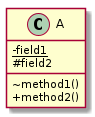
\includegraphics[width=3cm]{class-example.png}
  \centering
  \caption{diagramma delle classi realizzato con PlantUML}
\end{figure}
\begin{description}
  \item [Nomi e visibilità]: i nomi delle classi, dei campi dati e dei metodi andranno indicati in minuscolo e scritti in lingua inglese.
        Inoltre, come in un vero e proprio linguaggio di programmazione, in UML è possibile indicare la visibilità di una variabile o di un metodo:
        \begin{description}
          \item [-]: visibilità privata
          \item [\#]: visibilità protetta
          \item [+]: visibilità pubblica
          \item [\textasciitilde]: visibilità a livello di package.
        \end{description}
  \item[Altre convenzioni]:
        \begin{itemize}
          \item I campi dati e i metodi statici devono essere sottolineati.
          \item Utilizzare \textit{{abstract}} per indicare classi astratte.
          \item Fare uso di \textit{<<interface>>} per indicare interfacce.
          \item Il tipo delle variabili e il tipo di ritorno va posto dopo il nome della variabile o del metodo in questione. Ad esempio:
                \begin{center}
                  \textit{-field1: String} \\\textit{+method1: int}
                \end{center}
        \end{itemize}
  \item [Relazioni]: una relazione di dipendenza indica una dipendenza logica presente tra due elementi del diagramma e si ha quando la modifica di un oggetto implica il cambiamento di un altro oggetto.
        Esistono molteplici tipi di dipendenze e ognuna induce differenti gradi di dipendenza tra gli oggetti.
        Compito del progettista sarà quello di minimizzare il numero di dipendenze, utilizzandole solo ove necessario al fine di attribuire un valore aggiunto al significato del proprio diagramma.
        Di seguito verranno elencate i tipi di relazioni di dipendenza possibili, ordinati per grado di dipendenza crescente.
        \begin{description}
          \item [Dipendenza]: la dipendenza può verificarsi in due casi:
                \begin{itemize}
                  \item Una classe A ha un metodo che riceve in input un'istanza di B.
                  \item Una classe A crea un oggetto di tipo B.
                \end{itemize}
                Inoltre, per indicare il tipo di dipendenza useremo principalmente due parole chiave:
                \begin{description}
                  \item [\textit{<<call>>}]: A invoca operazioni di B.
                  \item [\textit{<<create}]: A crea istanze di B.
                \end{description}
                La dipendenza si indica con una freccia tratteggiata come illustrato nell'immagine sottostante.
                \begin{figure}[H]%
                  \label{fig:dipendenza}
                  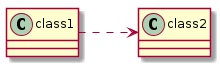
\includegraphics[width=5cm]{dipendenza.png}
                  \centering
                  \caption{Esempio di relazione di dipendenza}
                \end{figure}
          \item [Associazione]: l'associazione si verifica quando un oggetto di classe A ha un campo dati di tipo B.
                L'associazione si indica con una linea continua come nell'immagine sottostante:
                \begin{figure}[H]%
                  \label{fig:associazione}
                  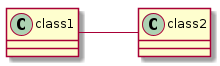
\includegraphics[width=5cm]{associazione.png}
                  \centering
                  \caption{Esempio di relazione di associazione}
                \end{figure}
          \item [Aggregazione]: l'aggregazione prevede che una classe di tipo A crei esplicitamente tramite il proprio costruttore degli oggetti di tipo B.
                L'aggregazione si rappresenta tramite una linea continua e un diamante che sta graficamente dalla parte di chi crea la dipendenza. Ad esempio:
                \begin{figure}[H]%
                  \label{fig:aggregazione}
                  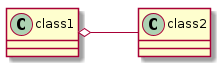
\includegraphics[width=5cm]{aggregazione.png}
                  \centering
                  \caption{Esempio di relazione di aggregazione}
                \end{figure}
          \item [Composizione]: la composizione è una forma di aggregazione più forte e si ha quando un oggetto di classe A gestisce completamente gli oggetti di tipo B.
                La composizione si rappresenta allo stesso modo dell'aggregazione, ma a differenza di quest`ultima il diamante è colorato di nero.
                \begin{figure}[H]%
                  \label{fig:composizione}
                  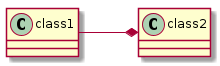
\includegraphics[width=5cm]{composizione.png}
                  \centering
                  \caption{Esempio di relazione di composizione}
                \end{figure}
          \item [Ereditarietà]: l'ereditarietà si ha quando un classe B deriva da una classe di tipo A.
                Ovviamente è preferibile ereditare da classi astratte o interfacce, mentre l'ereditarietà da tipi concreti sarebbe in ogni caso da evitare. Si rappresenta così:
                \begin{figure}[H]%
                  \label{fig:ereditarieta}
                  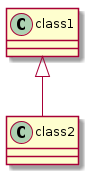
\includegraphics[width=2.1cm]{ereditarieta.png}
                  \centering
                  \caption{Esempio di relazione di ereditarietà}
                \end{figure}
        \end{description}
  \item [Molteplicità]: la molteplicità è uno strumento che permette di specificare quanti oggetti posso fare parte dell'associazione.
        Ogni molteplicità è una sigla costituita da numeri e simboli.
        Elenchiamo quelle di cui i progettisti dovranno fare uso:
        \begin{description}
          \item [1]: una classe A ha una e una sola istanza di classe di B associata.
          \item [0..1]: una classe A può avere zero o una istanze di classe B associata.
          \item [0..*]: una classe A può avere zero o più istanza di classe B associata.
          \item [*]: una classe A deve avere più istanze di B associate.
        \end{description}
\end{description}

\subparagraph{Diagrammi di package}%
\label{subp:diagrammi_di_package}
I diagrammi di package sono utili per rappresentare elementi appartenenti ad uno stesso namespace.
Hanno un'etichetta che identifica il nome, il quale deve essere in minuscolo e in inglese e possono contenere al loro interno altri package o classi.
Inoltre le dipendenze tra package si indicano con frecce tratteggiate e dovrebbero tutte seguire la medesima direzione.
\begin{figure}[H]%
  \label{fig:package}
  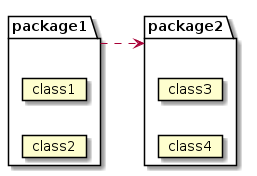
\includegraphics[width=5cm]{package.png}
  \centering
  \caption{diagramma dei package realizzato con PlantUML}
\end{figure}

\subparagraph{Diagrammi delle attività}%
\label{diagrammi_delle_attivita}%
I diagrammi delle attività rappresentano l'insieme delle azioni che ne costituiscono il funzionamento. Un tipico diagramma delle attività in PlantUML è:
\begin{figure}[H]%
  \label{fig:attività}
  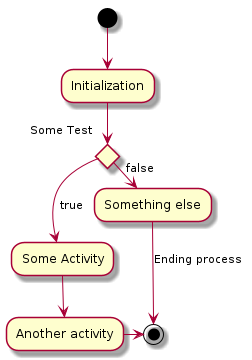
\includegraphics[width=5cm]{attivita.png}
  \centering
  \caption{diagramma delle attività realizzato con PlantUML}
\end{figure}
Gli elementi essenziali che li compongono sono:
\begin{itemize}
  \item Nodo iniziale
  \item Nodo finale
  \item Nodi di Branching
  \item Nodi di merge
  \item Fork e join.
\end{itemize}
I diagrammi di attività si basano sulla produzione e consumo di token.
Ogniqualvolta inizia il flusso di esecuzione e quindi ci trova nel nodo iniziale si genera un token.
Branching e merging rispettivamente producono e consumano un token, la fork produce un token per ogni processo in parallelo in esecuzione mentre la join li consuma tutti e ne genera uno.
Infine il nodo finale consuma tutti i token.
Altri elementi che possono essere utilizzati per realizzare diagrammi di attività più precisi sono:
\begin{itemize}
  \item Swimlanes
  \item Segnali
\end{itemize}
\begin{description}
  \item[Nodo iniziale]: il nodo iniziale è presente in ogni diagramma e delinea il punto di inizio di ogni diagramma delle attività. In PlantUML lo si rappresenta mediante un cerchio colorato di nero come nella figura:
        \begin{figure}[H]%
          \label{fig:nodo_iniziale}
          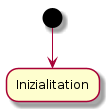
\includegraphics[width=3cm]{nodo-iniziale.png}
          \centering
          \caption{Esempio di nodo iniziale}
        \end{figure}
  \item[Nodo finale]: il nodo finale è presente in ogni diagramma e rappresenta il termine del flusso di esecuzione.
        In plantuml lo si raffigura come un cerchio contenente un altro cerchio colorato di nero:
        \begin{figure}[H]%
          \label{fig:nodo_finale}
          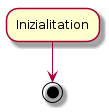
\includegraphics[width=3cm]{nodo-finale.png}
          \centering
          \caption{Esempio di nodo finale}
        \end{figure}
  \item[Nodi di branching]: i nodi di branching modellano delle decisioni.
        Hanno una guardia che indica quale test deve essere soddisfatto che si indica tramite un etichetta da affiancare al nodo di branching.
        Tali nodi si raffigurano mediante rombi vuoti e generalmente distinguono due branch:
        \begin{figure}[H]%
          \label{fig:nodo_di_branch}
          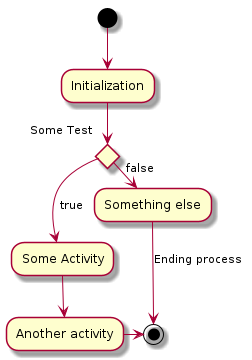
\includegraphics[width=5cm]{nodo-di-branch.png}
          \centering
          \caption{Esempio nodo di branching}
        \end{figure}
  \item[Nodi di merge]: i nodi di merge sono il punto in cui i rami generati da un nodo di branching tornano ad unirsi.
        Hanno la stessa rappresentazione dei nodi di branching.
        \begin{figure}[H]%
          \label{fig:nodo_di_merge}
          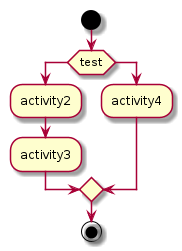
\includegraphics[width=5cm]{nodo-di-merge.png}
          \centering
          \caption{Esempio di nodo di merge}
        \end{figure}
  \item[Fork e join]: Fork e join sono necessari a rappresentare l'esecuzione parallela e concorrente.
        Ogniqualvolta il flusso di esecuzione incontra una fork il flusso di esecuzione diventa pari al numero di frecce uscenti dalla fork.
        Non è possibile terminare il flusso con più linee di esecuzione contemporaneamente attive ma è necessario che ci sia successivamente una join che ripristini l'unico flusso iniziale.
        Fork e join si rappresentano allo stesso modo, tramite una barra orizzontale colorata di nero. Ad esempio:
        \begin{figure}[H]%
          \label{fig:fork_e_join}
          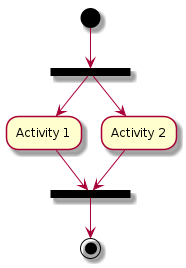
\includegraphics[width=5cm]{fork-e-join.png}
          \centering
          \caption{Esempio di fork e join}
        \end{figure}
  \item[Swimlanes]: Le Swimlanes sono strutture da poco introdotte in PlantUML che rendono esplicito di chi è la responsabilità nell'esecuzione. Si rappresentano così:
        \begin{figure}[H]%
          \label{fig:swimlanes}
          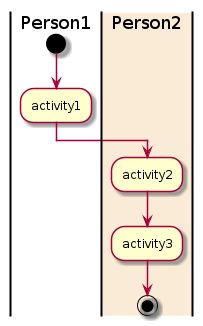
\includegraphics[width=5cm]{swimlanes.png}
          \centering
          \caption{Esempio di swimlanes}
        \end{figure}
  \item[Segnali]: I segnali servono per gestire eventi.
        PlantUML non offre un buon supporto per i segnali e ne offre una versione in beta.
        Ne esistono di due tipi:
        \begin{itemize}
          \item Segnali di input
          \item Segnali di output.
        \end{itemize}
  \item [Input]: i segnali di input aspettano una risposta proveniente dall'esterno.
        Possono essere la prima azione del diagramma.
        Si rappresentano così:
        \begin{figure}[H]%
          \label{fig:input}
          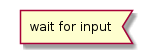
\includegraphics[width=5cm]{input.png}
          \centering
          \caption{Esempio segnale di input}
        \end{figure}
  \item [Output]: i segnali di output chiedono che venga inserito un input dall'esterno.
        Inoltre non possono essere la prima azione del diagramma.
        La loro rappresentazione è la seguente:
        \begin{figure}[H]%
          \label{fig:segnale_di_output}
          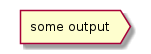
\includegraphics[width=5cm]{output.png}
          \centering
          \caption{Esempio segnale di output}
        \end{figure}
\end{description}

\subparagraph{Diagrammi di sequenza}%
\label{subp:diagrammi_di_sequenza}
I diagrammi di sequenza rappresentano dettagliatamente come gli oggetti interagiscono tra di loro mediante messaggi.
Ogni entità del diagramma è collegata mediante una linea tratteggiata verticale ad un'altra entità con lo stesso contenuto.
Tale linea indica il passare del tempo.
Le entità del diagramma si scambiano messaggi sotto forma di frecce che assumono una diversa struttura a seconda del tipo di messaggio che si sta inviando.
Segue un elenco delle tipologie di messaggi che due entità possono scambiarsi:
\begin{description}
  \item [Messaggio sincrono]: corrisponde alla chiamata di un metodo dal quale si attende un valore di ritorno.
        Lo si indica con una freccia continua nera piena accompagnata da un'etichetta contenente il tipo di metodo chiamato nella forma \textit{nomeMetodo (listaParametri)} dove la firma del metodo deve essere in lingua inglese e la lista di parametri deve essere nella forma \textit{nomeParametro1:tipo1, nomeParametro2:tipo2,\ldots}.
  \item [Messaggio asincrono]: corrisponde alla chiamata di un metodo dal quale non si attende nulla.
        Lo si indica con una freccia nera non piena accompagnata da un'etichetta identica a quella utilizzata per messaggi sincroni.
  \item [Messaggio di ritorno]: corrisponde ad un messaggio contenente il valore ritornato dalla chiamata di un metodo.
        Lo si indica con una freccia tratteggiata nera non piena accompagnata da un'etichetta contenente il tipo di valore ritornato.
  \item [Messaggio di creazione]: rappresenta un messaggio che chiede la creazione di un nuovo oggetto.
        Lo si indica con una freccia tratteggiata non piena seguita da un rettangolo contenente l'oggetto creato e accompagnata da un'etichetta contenente la parola \textit{<<create>>}.
  \item [Messaggio di distruzione]: rappresenta un messaggio che chiede la distruzione di un oggetto.
        Lo si indica con con una linea nera  seguita da una X e accompagnata da un'etichetta contenente la parola \textit{<<destroy>>}.
\end{description}
Un esempio di diagramma di sequenza corretto realizzato con PlantUML è il seguente:
\begin{figure}[H]%
  \label{fig:sequenza}
  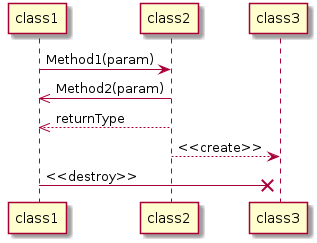
\includegraphics[width=7cm]{sequenza.png}
  \centering
  \caption{diagramma di sequenza realizzato con PlantUML}
\end{figure}
È possibile inoltre utilizzare delle cosiddette barre di attivazione per rendere immediatamente visibile a chi osserva il diagramma quando un'entità è attiva.
L`uso delle barre di attivazione non è obbligatorio ma è fortemente consigliato.
Il diagramma di prima con le barre di attivazione apparirebbe così:
\begin{figure}[H]%
  \label{fig:barre_attivazione}
  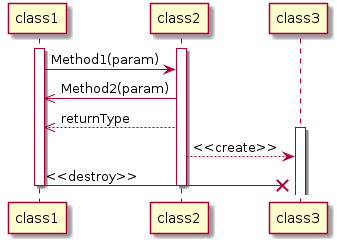
\includegraphics[width=7cm]{barre-attivazione.png}
  \centering
  \caption{Esempio barre di attivazione}
\end{figure}
Per modellare in maniera approfondita le interazioni fra oggetti è consigliato ai progettisti l'uso dei frame d'interazione introdotti in UML 2.
Tali frame si rappresentano come dei rettangoli a cui viene associata un'etichetta che indica il tipo di frame d'interazione.
Un esempio di diagramma di sequenza con i frame d'interazione è il seguente:
\begin{figure}[H]%
  \label{fig:frame_di_interazione}
  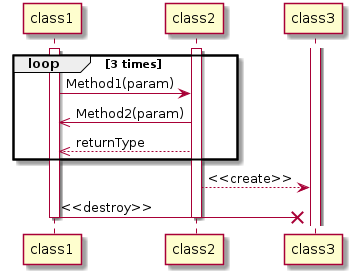
\includegraphics[width=7cm]{frame-interazione.png}
  \centering
  \caption{Esempio frame di interazione}
\end{figure}
Esistono diverse etichette per identificare i frame d'interazione. I progettisti dovranno attenersi alle seguenti:
\begin{description}
  \item [Alt]: indica frammenti alternativi che verranno eseguiti solo se la guardia è verificata.
  \item [Opt]: indica un frammento che viene eseguito solo se la condizione specificata è verificata.
  \item [Par]: indica frammenti da eseguire in parallelo.
  \item [Loop]: indica che il frammento può essere eseguito più volte, la base dell'iterazione è indicata dalla guardia.
  \item [Region]: indica una sezione critica. Il frammento può essere eseguito da un solo thread.
  \item [Neg]: indica un'interazione non valida.
  \item [Ref]: si riferisce ad un'interazione definita in una diagramma.
  \item [Ad]: si utilizza per racchiudere un intero diagramma di sequenza.
\end{description}

\paragraph{Aggiunta del codice}%
\label{par:aggiunta_codice}
Lo sviluppatore per aggiungere una funzionalità o semplicemente del codice deve attenersi alla seguente procedura:
\begin{itemize}
  \item aprire una branch da master nella repository in cui si vuole aggiungere la funzionalità e aprire una pull-request dalla branch appena creata
  \item implementare la funzionalità seguendo le regole definite dagli strumenti di supporto per la codifica
  \item implementare i test per la funzionalità e assicurarsi che siano rispettati i vincoli imposti dagli strumenti di supporto ai test di unità
  \item richiedere una review del codice
  \item se la review ha esito negativo sistemare i problemi rilevati e in seguito procedere con l'approvazione del codice e quindi con il merge del branch nel ramo master della repository.
\end{itemize}


% subs:procedure (end)

% subp:indentazione (end)

%\paragraph{Testing}%
%\label{par:testing}

\subsubsection{Strumenti di supporto}%
\label{subs:strumenti_di_supporto}

\paragraph{Strumenti utilizzati nella stesura della documentazione}%
\label{par:strumenti_utilizzati_nella_stesura_della_documentazione}

\subparagraph{PlantUML}%
\label{subp:plantuml}
Per la costruzione dei diagrammi UML il team ha deciso di utilizzare \glossario{PlantUML}\@.
È un software open source che permette la costruzione di diagrammi UML a partire dalla scrittura di codice in un linguaggio di markup dedicato. GruppOne ha valutato positivamente tale strumento in quanto:

\begin{itemize}
  \item Gli aspetti grafici di costruzione dei diagrammi sono demandati al software sottostante.
  \item La sua natura testuale e dichiarativa permette di attuare un versionamento efficace dei diagrammi attraverso strumenti già in uso dal team.
  \item Permette di scrivere agevolmente i diagrammi dei casi d'uso, delle classi, di sequenza e di package.
\end{itemize}

In seguito a difficoltà nell'utilizzo del package apposito di \LaTeX{}, abbiamo deciso di pre-compilare separatamente i diagrammi utilizzando le funzionalità esposte dalla \glossario{Command Line Interface} di PlantUML\@.

Posizionarsi nella cartella contenente la documentazione di progetto ed eseguire il comando:

\begin{minted}{bash}
  java \
    -jar \
    $PLANTUML_JAR \
    -checkmetadata \
    -charset UTF-8 \
    -x **/commons/style/*.pu \
    -o img \
    **/**.pu
\end{minted}

La corretta esecuzione del comando richiede di aver impostato la variabile d'ambiente \verb|PLANTUML_JAR| al percorso completo del file \verb|plantuml.jar| reperito dal sito del progetto.

In questo modo vengono generate le immagini che sono effettivamente incluse nei documenti dal comando dato in~\ref{par:LaTeX}.

\href{https://plantuml.com/}{Sito web di PlantUML}
% subp:plantuml (end)

\subparagraph{Package pgfgantt}%
\label{subp:pgfgantt}

Per i diagrammi di Gantt il gruppo ha scelto di utilizzare pgfgantt, un package disponibile per \LaTeX{} che sfrutta il linguaggio \glossario{PGF} e il rispettivo omonimo interprete.
PGF è in grado di produrre rappresentazioni grafiche vettoriali, e pgfgantt fornisce dei comandi \TeX{} che fungono da astrazioni per le direttive di basso livello.
Un diagramma di Gantt viene quindi costruito attraverso uno o più comandi di titolo, seguiti da una combinazione di comandi specifici per inserire gruppi, ``barre'' (cioè attività) o milestone, oppure per collegare due elementi.

L'integrazione dei diagrammi nel documento avviene durante la compilazione del documento effettuata attraverso il comando dato in~\ref{par:LaTeX}.

\href{http://texdoc.net/texmf-dist/doc/latex/pgfgantt/pgfgantt.pdf}{Link alla documentazione del pacchetto}
% subp:pgfgantt (end)

\subparagraph{ChkTex}%
\label{subp:chktex}
Per rilevare errori tipografici e sintattici il gruppo ha scelto di utilizzare \glossario{ChkTex} un \glossario{linter} per \LaTeX{}.

\href{https://www.nongnu.org/chktex/}{Link allo strumento}
% subp:chktex (end)


\paragraph{Code editor utilizzati}%
\label{par:code_editor}

\subparagraph{MS-Visual Studio Code}%
\label{subp:vscode}
Come \glossario{code editor} è stato scelto Visual Studio Code.
Visual Studio Code è un editor di codice sorgente sviluppato da Microsoft per Windows, Linux e macOS\@. Include supporto per debugging, un controllo per Git integrato, refactoring del codice, ecc. Offre inoltre supporto di prima classe e capacità avanzate paragonabili ad un IDE per quanto riguarda i linguaggi di programmazione JavaScript e TypeScript.

\href{https://code.visualstudio.com/}{Sito web di Visual Studio Code}
% subp:vscode (end)

\subparagraph{Stoplight Studio}%
\label{subp:stoplight_studio}
Per lo sviluppo della API è stato scelto Stoplight Studio.
Stoplight Studio offre una serie di funzionalità che coprono l'intero ciclo di vita dell'API di pre-produzione, dalla modellazione, al test, alla simulazione del funzionamento dell'API\@.

\href{https://stoplight.io/docs}{Documentazione di Stoplight}
% subp:stoplight_studio (end)

\paragraph{Ambienti di sviluppo utilizzati}%
\label{par:ambienti_di_sviluppo}

\subparagraph{IntelliJ IDEA}%
\label{subp:intellij}
Per la mobile app è stato scelto l'ambiente di sviluppo IntelliJ IDEA, un ambiente di sviluppo integrato (IDE) per il linguaggio di programmazione Java.

\href{https://www.jetbrains.com/idea/}{Sito web di IntelliJ IDEA}
% subp:intellij (end)

\paragraph{Analisi statica e dinamica}%
\label{par:analisi_statica_e_dinamica}

\subparagraph{SonarCloud}%
\label{subp:sonarcloud}
Per tutti i componenti è stato scelto di utilizzare SonarCloud.
SonarCloud è uno strumento in grado di segnalare bug e vulnerabilità e migliorare il flusso di lavoro grazie al concetto di Continuous Code Quality.

\href{https://sonarcloud.io/documentation}{Documentazione di SonarCloud}
% subp:sonarcloud (end)

\paragraph{Strumenti eseguiti da IntelliJ IDEA}%
\label{par:strumenti_eseguiti_da_Intellij_IDEA}

\subparagraph{Checkstyle}%
\label{subp:checkstyle}
Per lo sviluppo del server e della mobile app è stato scelto di utilizzare Checkstyle.
Checkstyle è uno strumento di sviluppo che aiuta gli sviluppatori a scrivere codice Java che aderisce a uno standard di codifica. Automatizza il processo di controllo del codice e questo lo rende ideale per i progetti che vogliono applicare uno standard di codifica.

\href{https://checkstyle.sourceforge.io/}{Link allo strumento}
% subp:checkstyle (end)

\subparagraph{Android Lint}%
\label{subp:androidlint}
Per lo sviluppo della mobile app è stato scelto di utilizzare Android Lint.
Android Lint è un strumento che analizza il progetto Android alla ricerca di potenziali buge possiede un'architettura indipendente dall'IDE, quindi integrabile con altri IDE, con altri strumenti di costruzione e anche con sistemi di integrazione continua.

\href{https://developer.android.com/studio/write/lint}{Link allo strumento}
% subp:androidlint (end)

\paragraph{Strumenti eseguiti da VS Code e nella pipeline di Continuous Integration:}%
\label{par:strumenti_eseguiti_da_vscode_e_ci}

\subparagraph{Eslint}%
\label{subp:eslint}
Per lo sviluppo della web-app è stato scelto di utilizzare Eslint.
ESLint analizza staticamente il codice per trovare rapidamente i problemi ed è possibile eseguire ESLint come parte della pipeline di integrazione continua. Molti problemi rilevati da ESLint possono inoltre essere risolti automaticamente e le correzioni avvengono rispettando la sintassi, quindi non si verificano errori introdotti dagli algoritmi tradizionali di ricerca e sostituzione.

\href{https://eslint.org/}{Sito web di ESLint}
% subp:eslint (end)

\subparagraph{Stylelint}%
\label{subp:stylelint}
Per lo sviluppo della web-app è stato inoltre scelto di utilizzare Stylelint.
Stylelint è un linter che aiuta a evitare errori e ad applicare convenzioni nei fogli di stile.

\href{https://stylelint.io/}{Sito web di Stylelint}
% subp:stylelint (end)

\subparagraph{Prettier}%
\label{subp:prettier}
Per lo sviluppo della web-app è stato inoltre scelto di utilizzare un code formatter: Prettier.
Prettier è un formattatore di codice supponente. Applica uno stile coerente analizzando il codice e ristampandolo con le proprie regole che tengono conto della lunghezza massima della linea, andando a capo quando necessario senza alterare la semantica del codice.

\href{https://prettier.io/}{Sito web di Prettier}
% subp:stylelint (end)

\paragraph{Framework e SDK}%
\label{par:framework_sdk}

\subparagraph{Angular}%
\label{subp:angular}
Per lo sviluppo della web-application il gruppo ha deciso di appoggiarsi ad Angular, un framework per lo sviluppo di applicazioni web, il linguaggio utilizzato è Typescript.

\href{https://angular.io/docs}{Documentazione di Angular}

\subparagraph{Spring}%
\label{subp:spring}
Per sviluppare il server è stato scelto Spring, un framework open source per lo sviluppo di applicazioni in linguaggio Java, sono associati a Spring altri progetti che offrono funzionalità aggiuntive al framework.

\href{https://spring.io/}{Sito di Spring}

\subparagraph{Android SDK}%
\label{subp:android_sdk}
Il gruppo per sviluppare l'applicazione mobile richiesta dal capitolato ha scelto di avvalersi di Android SDK, un framework per lo sviluppo software android che include molti strumenti per facilitare lo sviluppo di applicazioni android.
È associato ad IntelliJ idea nello sviluppo della mobile app\dots

\href{https://developer.android.com/guide}{Guida di Google allo sviluppo Android}

\paragraph{Framework di testing}%
\label{par:framework_test}
Per effettuare i test di unità all'interno della web application è stato scelto Jasmine, un framework per il test orientato verso il behavior-driven-development.
Associato all'ambiente di test Karma costituisce la suite di Angular per i test di unità.

\href{https://jasmine.github.io/}{Documentazione di Jasmine}

\subparagraph{Protractor}%
\label{subp:protractor}
Per effettuare i test e2e è stato scelto protractor, un framework per i test e2e in grado di simulare le interazioni dell'utente con la web application.
Viene integrato automaticamente con Angular.

\href{https://www.protractortest.org/}{Sito web di Protractor}

\subparagraph{JUnit}%
\label{subp:junit}
Per effettuare i test di unità nello sviluppo del server e della applicazione mobile il gruppo ha scelto di utilizzare JUnit, un framework di unit testing per il linguaggio Java.

\href{https://junit.org/junit4/}{Sito web di JUnit}

\subparagraph{Mockito}%
\label{subp:mockito}
Per lo sviluppo dell'applicazione mobile e del server è stato scelto Mockito, un mocking framework per Java.

\href{https://site.mockito.org/}{Documentazione di Mockito}

\subparagraph{Espresso}%
\label{subp:espresso}
Per sviluppare l'applicazione mobile il gruppo si appoggia a Espresso, un framework per i test di sistema nello sviluppo android.

\href{https://developer.android.com/training/testing/espresso}{documentazione di Espresso}

% \subparagraph{Cucumber}%
% \label{subp:pgfgantt} test autoesplicativi

\paragraph{Gestori delle dipendenze}%
\label{par:gestori_dipendenze}

\subparagraph{Node Package Manager}%
\label{subp:npm}
Per gestire le dipendenze della web application il gruppo si appoggia a npm, il gestore delle dipendenze di Node.js.

\href{https://www.npmjs.com/}{Sito web di npm}

\subparagraph{Gradle}%
\label{subp:gradle}
Per gestire le dipendenze della web application il gruppo si appoggia a npm,
Gradle è un sistema per l'automazione dello sviluppo che introduce un domain-specific language basato su Groovy.
Gradle supporta sviluppi incrementali determinando in modo intelligente quali parti del build tree sono aggiornate (``up-to-date''), in modo che tutti i processi che dipendono solo da quelle parti non avranno bisogno di essere eseguiti nuovamente; così facendo, il software riduce significativamente il tempo di costruzione del progetto.

\href{https://gradle.org/}{Sito web di Gradle}
\end{document}
